% THIS IS SIGPROC-SP.TEX - VERSION 3.1
% WORKS WITH V3.2SP OF ACM_PROC_ARTICLE-SP.CLS
% APRIL 2009
%
% It is an example file showing how to use the 'acm_proc_article-sp.cls' V3.2SP
% LaTeX2e document class file for Conference Proceedings submissions.
% ----------------------------------------------------------------------------------------------------------------
% This .tex file (and associated .cls V3.2SP) *DOES NOT* produce:
%       1) The Permission Statement
%       2) The Conference (location) Info information
%       3) The Copyright Line with ACM data
%       4) Page numbering
% ---------------------------------------------------------------------------------------------------------------
% It is an example which *does* use the .bib file (from which the .bbl file
% is produced).
% REMEMBER HOWEVER: After having produced the .bbl file,
% and prior to final submission,
% you need to 'insert'  your .bbl file into your source .tex file so as to provide
% ONE 'self-contained' source file.
%
% Questions regarding SIGS should be sent to
% Adrienne Griscti ---> griscti@acm.org
%
% Questions/suggestions regarding the guidelines, .tex and .cls files, etc. to
% Gerald Murray ---> murray@hq.acm.org
%
% For tracking purposes - this is V3.1SP - APRIL 2009


\documentclass{acm_proc_article-sp}

\usepackage{algorithm2e}
\usepackage{algorithmic}

\begin{document}

\title{A Concept-based Approach for Query Suggestion}

\numberofauthors{3}
\author{
\alignauthor
Jack Sun\\
       \affaddr{Shanghai Jiao Tong University}\\
       \affaddr{Shanghai, China}\\
       \email{jacksunwei@gmail.com}
\alignauthor
Franky\\
       \affaddr{Shanghai Jiao Tong University}\\
       \affaddr{Shanghai, China}\\
       \email{franky.id@gmail.com}
\alignauthor
Kenny Q. Zhu\\
       \affaddr{Shanghai Jiao Tong University}\\
       \affaddr{Shanghai, China}\\
       \email{kzhu@cs.sjtu.edu.cn}
}

\maketitle
\begin{abstract}
Improving the user experience in using search engine, 
we consider the task of concept-based query suggestion, 
in which the user query contains one or more abstract 
concepts. For instance, a word ``movies'' in user query may 
be considered as a concept which can be instantiated into 
``indiana jones'' or ``star wars''. We present a query 
suggestion approach that provides the user with more 
specific queries taken from query log, with each query 
contains instantiation of concepts found in user query. 
We utilize Probase, a taxonomic knowledge base, to find 
the appropriate instantiation. A number of similarity 
scores that include edit distance, word distance, and 
typicality distance are used to measure the relevancy 
of replacement queries. Quality of the queries are also 
considered, using the frequencies and the number of 
click-throughs performed for those queries. The resulting 
queries are then showed to user to improve the search 
experience and helping them to form a better and specific 
query. \textit{Our evaluation shows that the resulting 
queries have high/acceptable relevancy to the user query 
and may represent user intention when searching for certain 
vague concepts.}
\end{abstract}

% A category with the (minimum) three required fields
\category{H.3.3}{Information Search and Retrieval}{Query 
formulation, Retrieval Models, Search Process, Selection 
Process}

\terms{Algorithms, Experimentation}

\keywords{Query rewriting, query substitution, concept-based 
search, topic search, Probase} % NOT required for Proceedings

% introduction
\section{Introduction}

Protein$-$protein interactions (PPIs) are of central importance for the majority of biological functions, such as signal transduction, metabolic pathways, molecular dynamics, and protein networks\cite{Hoffmann.Krallinger.ea:2005}, for they serve as the most fundamental building blocks of the entire interacademic systems of any organisms. Collecting data on pairwise interaction relationships is essential for multiple purpose, including identification of modules with certain functionality\cite{Spirin.Mirny.03}, mapping diseases to dominated genes\cite{Ideker.Sharan.08}, and after all, understanding wholistic metabolic/genetic networks from a system biology perspective.

A lot of databases have been built to store protein and genetic interactions from major model organism species and are available in various standardized formats, such as MINT\cite{Zanzoni.Montecchi-Palazzi.ea:2002}, BIND\cite{Bader.ea:2003}, BIOGRID\cite{DBLP:journals/nar/StarkBRBBT06}, etc. Among those mainstream databases, the data largely rely on voluntary reports by scientists or researchers, besides, comprehensive curation efforts become indispensable for the sake of accuracy. However, the amount of biology-related literatures with respect to protein interactions grows explosively and thus make it either impossible or impractical to manually detect PPI information anymore.

Considering huge amount of PPI information with great wealth hidden in published papers, in recent years, numerous mining techniques have been proposed that aim to extract PPI information automatically from free text, especially machine learning, information retrieval, and natural language processing\cite{DBLP:journals/bib/WinnenburgWPDS08}.These approaches can be roughly categorized into three classes: co$-$occurrence, rule$-$based, and machine learning. 

Co$-$occurrence is the approach with most simplicity and naivete. Just as its name implies, this method intends to find out pairs of proteins that co-occur in the same context. The scope of "same context" ranges from phrase, sentence, paragraph to whole abstract, even document. The underlying assumption is that whenever two proteins are mentioned together by authors, chances are high that there is some kind of relationship between them. However, however, in-context closeness even semantic relation does not necessarily represent actual biological interaction. As a consequence, a large fraction of candidate pairs are mismatched inevitably, causing a high recall but low precision.

The second approach is rule-based extraction, in other words, pattern matching. There are many types of rules, most of them concern natural language processing (NLP). One way is to specify hand-crafted regular expressions before hand, which mostly lean on language usage preference. Besides, by using full or partial (shallow) parsing strategies, more information would be acquired, such as part-of-speech taggers, local dependencies between syntactic components, context-free grammar\cite{DBLP:journals/bioinformatics/TemkinG03}, and full sentence structure. Compared to co$-$occurrence, rule-based approach enjoy better precision but much lower recall. In addition, since the rules are usually derived from training data, that is to say, the improper choice of training data would be significantly lethal, therefore quality of extraction is invariably instable and may not applicable to other data.

The third and most commonly used approach use machine learning techniques, in this case, the task to extract protein$-$protein interactions turns out to be a binary classification problem. Each protein pairs are represented along with a set of features, which is associated with their context, then a well$-$defined classifier gives the answer whether the candidate protein pairs is classified to be qualified PPI. (TO BE FURTHER FILLED!!!)

In this paper, we introduce a general bootstrapping framework for Protein$-$protein interaction extraction from natural text.Our method differs from most of the previous works in three aspects:

(1)The extraction process is driven by only tiny fraction of training data, which are regarded as seed data. In each round, it would derive reliable patterns automatically from seed data, then extract more positive PPI pairs consequently, what's more, the seed data would be augmented by the newly extracted results with high confidence.

(2)multiple graph kernel. 

(3)various evaluation.




% overview of Probase
\section{Probase}
Probase is a probabilistic knowledge base, built by 
extracting pairs of \textit{isA} relationship of concepts 
from web pages. In Probase, concepts are stored in a 
taxonomic manner. Currently, it contains around 2.7 
million concepts that were extracted from more than 1 
billion web pages. A concept in Probase can be seen as 
a representation of object in real world. An instance 
can also be considered as a single concept, which cannot 
be instantiated into other concepts or instances. Figure 
\ref{fig:exampleProbase} shows the example for this relation.

\begin{figure}[h]
\centering
\includegraphics[scale=0.3]{images/Figure2}
\caption{Example of concepts and instances in Probase}
\label{fig:exampleProbase}
\end{figure}

We can see from this figure, that ``animals'', ``livestocks'', 
``reptiles'', ``snakes'', ``korean singers'' are regarded as 
concepts, and ``boa'' as an instance. A concept may be a 
subconcept of other concept, e.g. ``snakes'' is a subconcept 
of ``animals''.

The distinctive aspect of Probase compared with other knowledge 
bases is that, in Probase, the relation between a concept and 
subconcept or a concept and an instance is not defined in a strict 
well-defined manner. Each relation is given a probability value 
which measure the \textit{value} of the relationship. The first 
value called \textit{plausibility} value, measures how strong or 
certain we are that a concept and a subconcept is actually related. 
Take an example of pair (``animals'',``reptiles''). The plausibility 
value tells us how strong that the 'reptiles' is seen as 'animals' or 
how certain we are that 'reptiles' is indeed 'animals'. This degree 
of uncertainty is important since it represents how exactly the 
concepts in the real world is attached to each other.

Another value that is a subject of interest to us in this work is 
the \textit{typicality} value. It measures how strong the relation 
between a concept and an instance. We take use of this value as one 
of the components to measure the relevancy between the concepts in 
user query and the instances found in queries from query log. The 
value is derived as:
\[Typicality\textnormal{-}value(i, c) = \frac{n(i, c)}{n(c)+\alpha}\]
where $i$ is an instance and $c$ is a concept. The $n(i,c)$ is the 
frequency of the occurrence of instance $i$ and concept $c$ together 
in extracted pairs from web pages, and $n(c)$ is the frequency of the 
occurrence of concept $c$ in all pairs. The value $\alpha$ is used 
to smooth the score and to avoid the high typicality value of a 
concept $c$ that only have one instance $i$, which can be harmful 
if the relationship is supposed to be small. To show how typicality 
value can be used, take an example of an instance ``boa''. The 
typicality value of pair (``boa'',``snakes'') is 0.0138 while the pair 
(``boa'',``korean singers'') has typicality value of 0.00197. From 
this result, we can see that ``boa'' is more likely known as a name 
of a snake than as the name of a singer.
\\
\\


%439871 boa
%1720113 snakes
%973216 korean singers
%
%439871	61
%1720113	0.0138181818181818
%993835	0.00486144871171609
%973216	0.0019723865877712



% overall structure
\section{Overall Structure}
In essence, our system is to reorganize the search log according to the structure of concepts and use the reorganized
structure to quickly retrieve the matching historical queries and return them to user.

In order to achieve that, we divide our system into two parts. One is the offline part, responsible for precomputing the
index of search log. The other one is the online part, which can retrieve the index, rank the candidate queries and show
 results. As is shown in Fig. \ref{fig:overall-structure}, the two part is connected by the index of search log.

\begin{figure}[h]
\centering
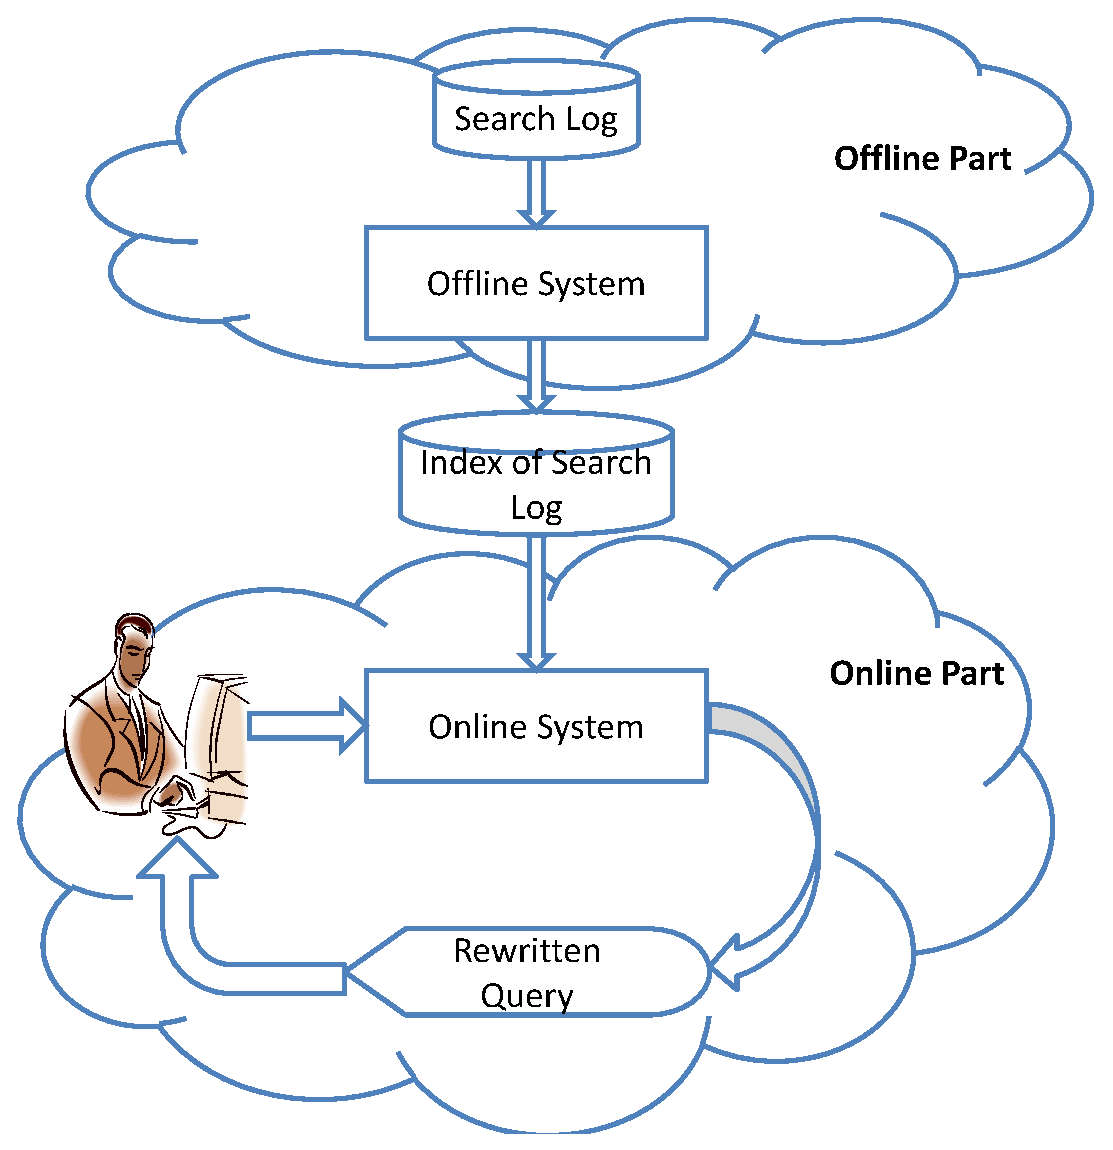
\includegraphics[scale=0.3]{images/overall}
\caption{Overall Structure of System}
\label{fig:overall-structure}
\end{figure}

% offline work
\section{Preprocessing}
In this step, our goal is to build an offline data structure according to Probase's taxonomy, so that the runtime system (search process) can quickly return queries that contain concepts found in user query. In brief, the preprocessing step is to generate a model file of inverted index that can provide an index from Probase concept to queries in query log.

The preprocessing step is performed in two steps - conceptualization and aggregation. First, we \textit{conceptualize} each instances found in each historical query from query log to some certain Probase concepts, resulting in an intermediate file with index from queries to concepts in the form of "\textit{query-id $\to$ concept-ids}". In the second step, we reorganize the intermediate file into an inverted index format from concept to queries in the form of \textit{"concept-id $\to$ query-ids"}.

\subsection{Conceptualization Step}
In this step, we aim at conceptualizing instances in historical queries. In order to achieve that, first, we parse the query into a sequence of \textit{keywords} and Probase instances. Then, we conceptualize each instance into Probase concepts using the \textit{isA} relationship information from Probase. We define a \textit{keyword} as a single word, which is neither an instance nor a concept in Probase.

The parsing process uses a similar algorithm with Parser, i.e. maximum-match algorithm (Algorithm \ref{alg:parse}), 
which will be presented later. For example, if we find a phrase 'president obama' and assuming that 'president', 
'obama', and 'president obama' are all valid instances in Probase. The algorithm will take the longest possible 
one - 'president obama' - as the recognized instance.

For conceptualizing instances, we use typicality information of each instance, which is a part of Probase. Each 
instance $i$ has a list of pairs ($c$, $t$), where $c$ denotes a Probase concept in which this instance can be 
conceptualized into and $t$ denotes a \textit{typicality} value of how likely the instance $i$ relate to the 
concept $c$.

At the end of this step, the system will produce an intermediate file for later step. Each line starts with a 
\textit{query-id} followed by \textit{instance-id} for instances found in the query, \textit{concept-id} of 
the super concept of the instance and the typicality value. The Fig. \ref{fig:conceptualization} shows how the 
intermediate file is organized.

\begin{figure}[h]
\centering
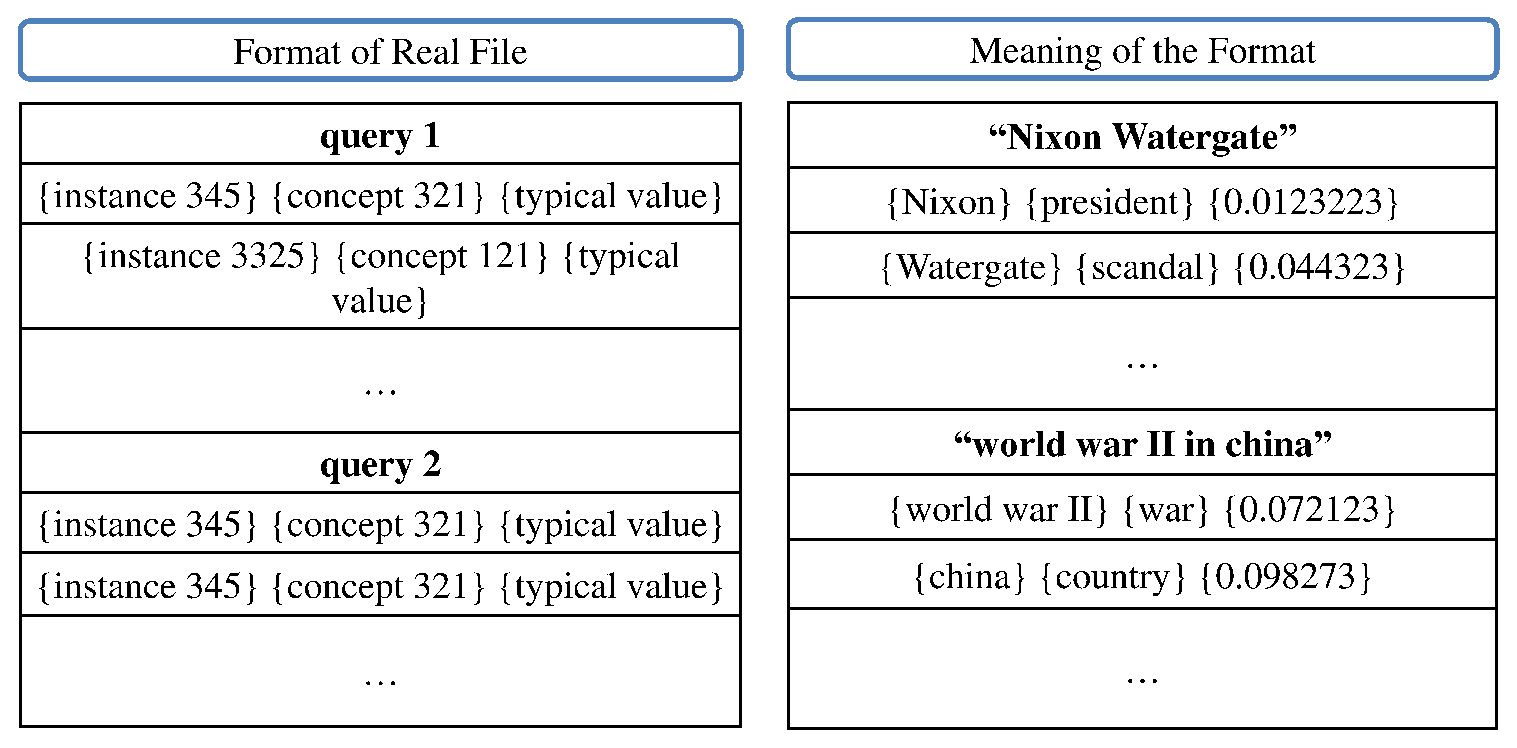
\includegraphics[scale=0.3]{images/conceptualization}
\caption{Format of Conceptualization Model File}
\label{fig:conceptualization}
\end{figure} 

\subsection{Aggregation Step}
We convert the format of the intermediate file produced in conceptualization step and produce the final aggregation 
file. The intermediate file is organized by unit of query, while the aggregation file is an inverted index organized 
by unit of concepts. The Fig. \ref{fig:aggregation} illustrates the format of the aggregation file.

\begin{figure}[h]
\centering
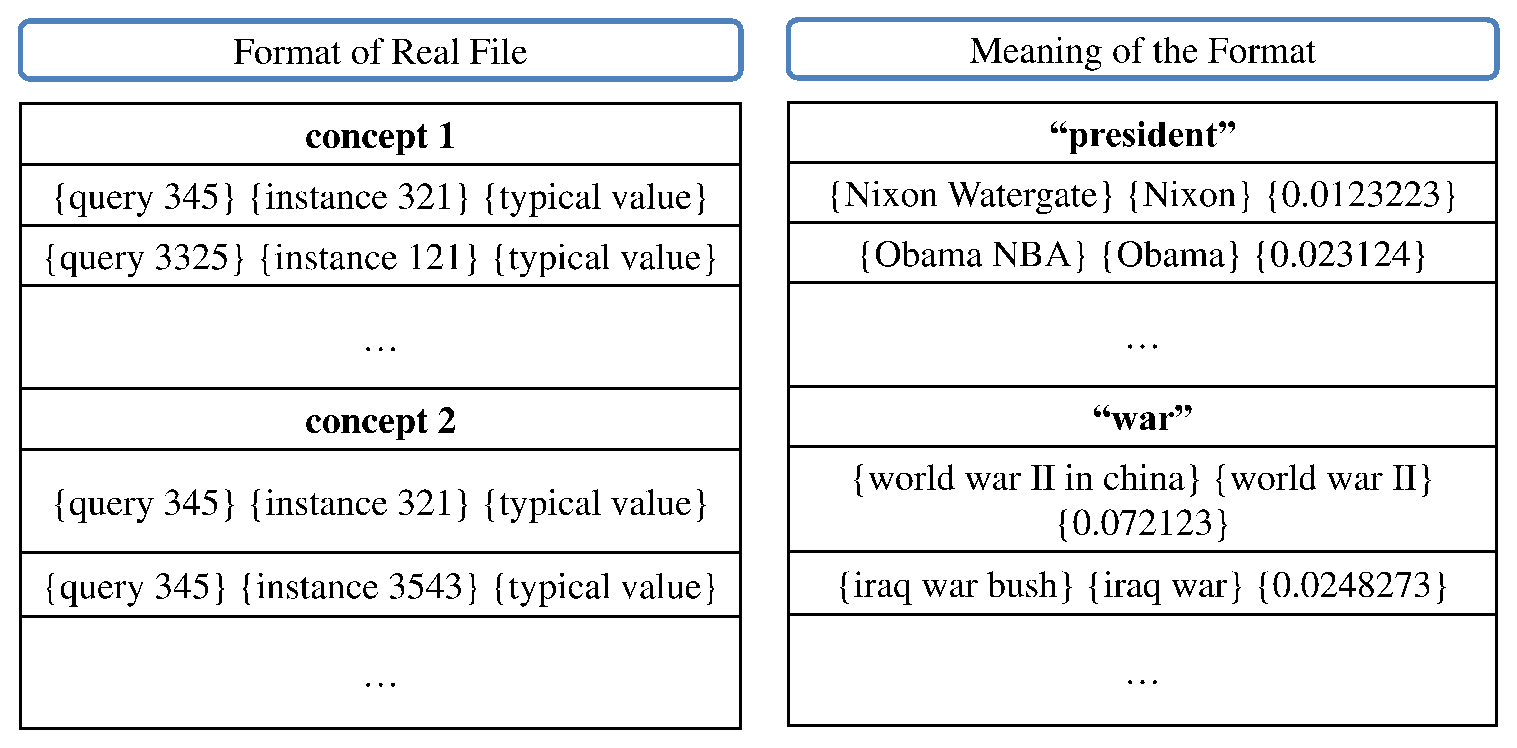
\includegraphics[scale=0.3]{images/aggregation}
\caption{Format of Aggregation Model File}
\label{fig:aggregation}
\end{figure} 

\subsection{Space Complexity Analysis}
\label{sec:spaceAnalysis}
In order to make a clear description, we define the following notations:

\begin{itemize}
  \item $n$: total number of historical queries in query log.
  \item $I_{hq}$: average number of Probase instances in each historical query.
  \item $C_I$: average number of Probase concepts, that a Probase instance can be conceptualized to.
\end{itemize}

Using the above notations, we can see that in average each historical query will be stored $I_{hq} \times C_I$ times in the aggregation file. Because there are $n$ queries in search log, the overall space complexity of aggregation file will be $O(I_{hq} \times C_I \times n)$. In this case, if we consider $I_{hq}$ and $C_I$ as constant, the overall space complexity of preprocessing will be $O(n)$, linear to the size of the query log.


% online processing
\section{Runtime System}
In this section, we would like to describe the runtime system of this project. The runtime system will interact with users, receiving a query from user and giving our suggested rewritten query. Figure \ref{fig:system} illustrate an overall structure of runtime system.

\begin{figure}
  \centering
  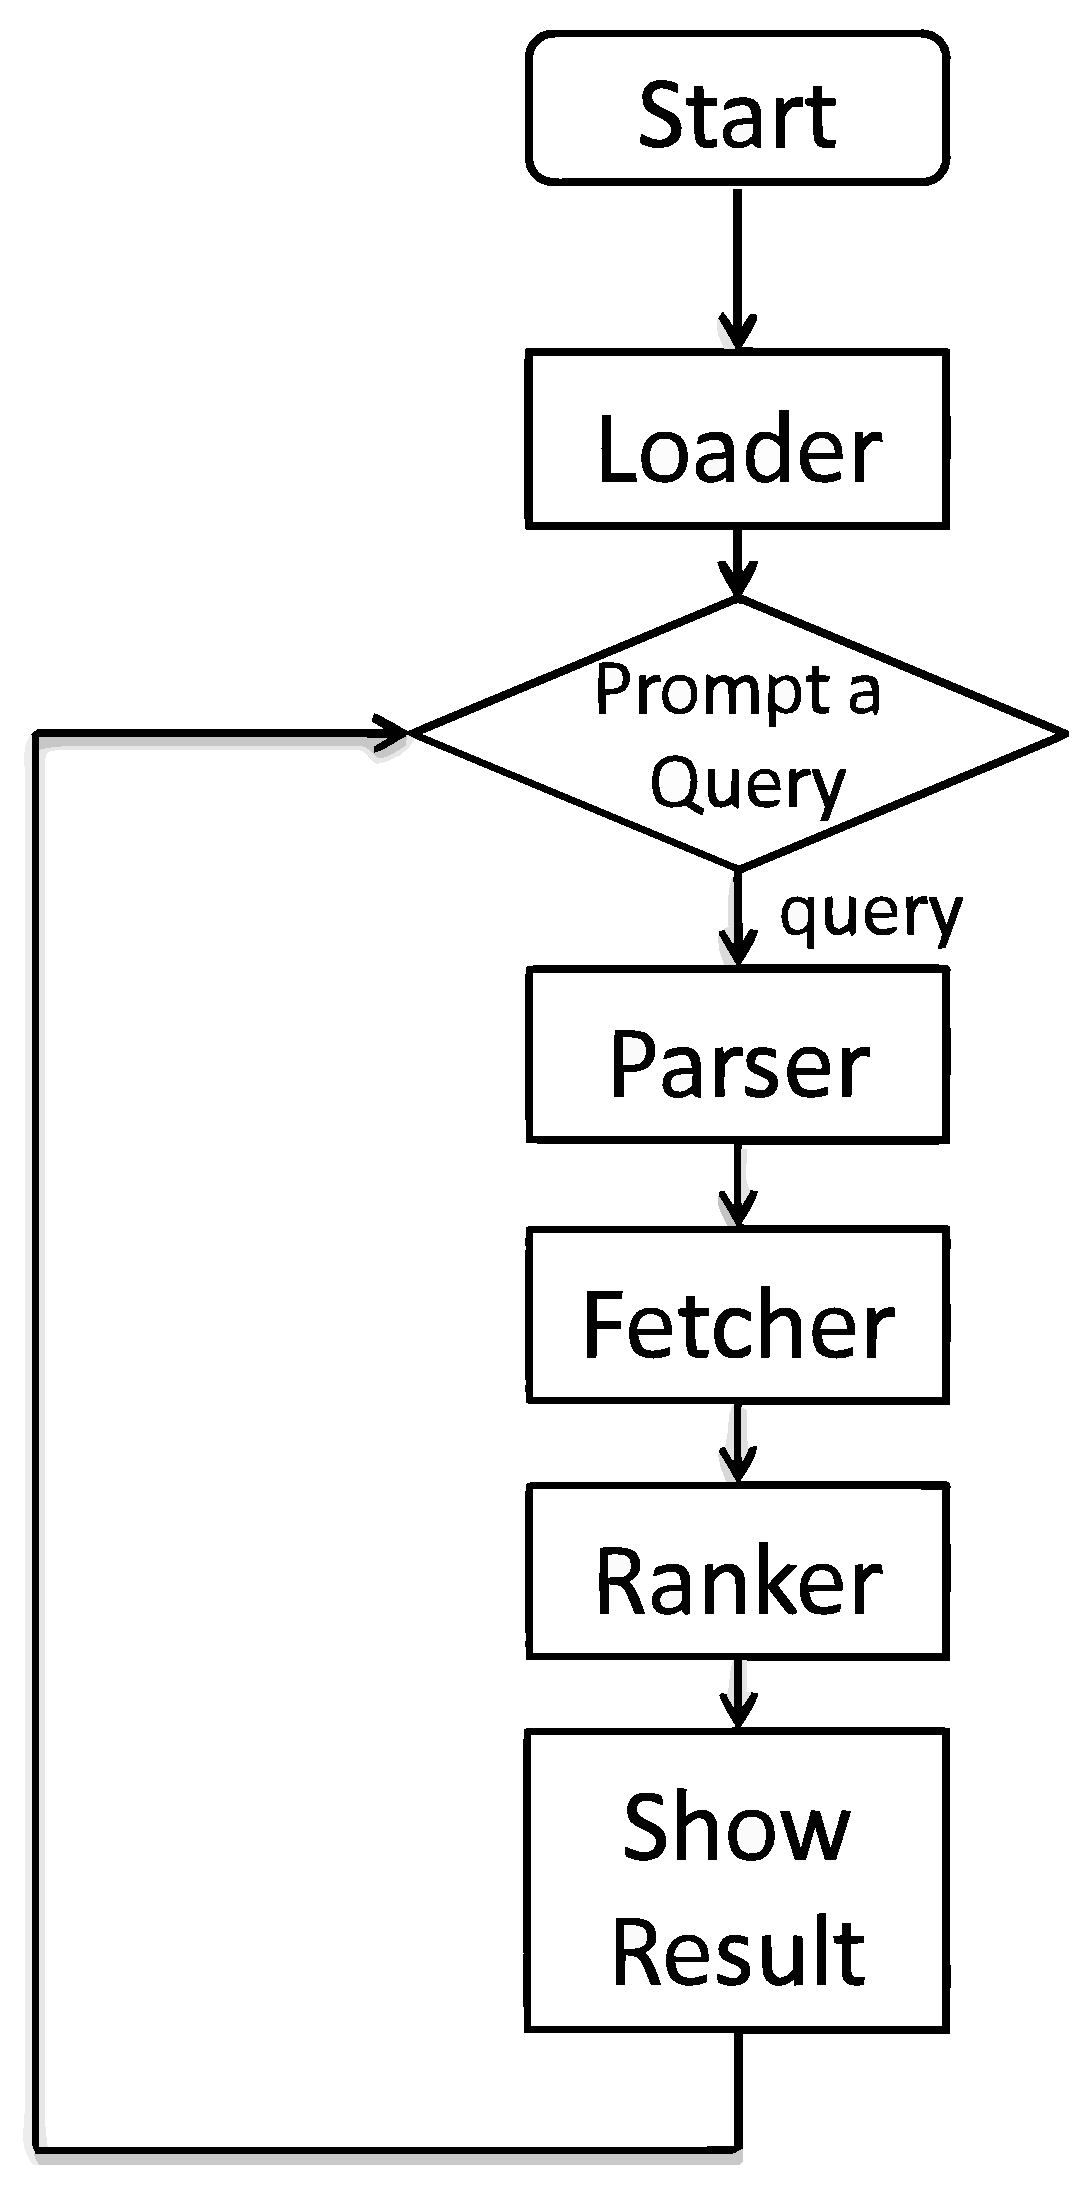
\includegraphics[scale=0.2]{images/system}
  \caption{Overall Structure of Runtime System}
  \label{fig:system}
\end{figure}

\subsection{Loader}
This module is started right after runtime system begins. \textbf{Loader} plays a role as a data provider. It loads necessary data into memory and caches regularly used disk-stored data. Such data includes but not limited:

\begin{itemize}
  \item Instance list and Concept list from Probase.
  \item All historical queries in search log.
  \item Aggregation file.
\end{itemize}

\subsection{Parser}
This module receives a string query from user and uses information from \textbf{Loader} to parse the query into a sequence of Probase concepts and keywords. The complete algorithm is listed in Algorithm \ref{alg:parse}.

\begin{algorithm}
\caption{Parsing Function}
\label{alg:parse}
\begin{algorithmic} [1]
  \REQUIRE a query Q;
  \ENSURE a sequence of concepts and keywords SEQ;

  \STATE $SEQ \Leftarrow PostagParser(Q)$ \\
  \COMMENT {use a postag parser to do word-splitting and postaging}
  \STATE $L \Leftarrow LengthOf(SEQ)$
  \FOR {$max = L$ to $1$}
    \FOR {$i = 0$ to $L - max$}
      \IF {no concept from $SEQ[i]$ to $SEQ[i+max]$}
        \STATE $Test \Leftarrow$ Link $SEQ[i]$ to $SEQ[i+max]$
      \ENDIF
      \IF {$Test$ is a concept}
        \STATE $SEQ[i] \Leftarrow Test$
        \STATE Mark $SEQ[i]$ as a concept
        \STATE Remove $SEQ[i+1]$ to $SEQ[i+max]$
        \STATE $L \Leftarrow L - max + 1$
      \ENDIF
    \ENDFOR
  \ENDFOR
  \RETURN $SEQ$
\end{algorithmic}
\end{algorithm}

\subsubsection{Time Complexity Analysis}
In the worst case, there are no concepts in the query. \textbf{Parser} has to test
\[(1+2+ \cdots +m) = \frac {m \times (m+1)} {2}\] times
, where $m$ is number of words in the query. Besides, the cost of each test is $O(1)$ because the test is based on hash algorithm. In total, the overall time complexity of \textbf{Parser} is $O(m^2)$.

\subsection{Fetcher}
This module receives concept list from \textbf{Parser} and get aggregation list of each concept from \textbf{Loader}. And then, Fetcher does an intersection work to these lists and turns one list of historical queries to next module. The complete algorithm is listed in Algorithm \ref{alg:fetch}.

\begin{algorithm}
\caption{Fetching Function}
\label{alg:fetch}
\begin{algorithmic} [1]
  \REQUIRE a sequence of concepts and keywords $SEQ$
  \ENSURE an intersected aggregation list of concepts

  \STATE $LIST \Leftarrow \varnothing$

  \FOR {$i = 1$ to $LengthOf(SEQ)$}
    \IF {$SEQ[i]$ is a concept}
      \STATE $C_i \Leftarrow$ fetch aggregation list of $SEQ[i]$ from \textbf{Loader}
      \STATE add $C_i$ to $LIST$
    \ENDIF
  \ENDFOR
  \RETURN $\bigcap_{i=1}^{\infty} C_i$, $C_i \in LIST$
\end{algorithmic}
\end{algorithm}

\subsubsection{Time Complexity Analysis}
The routine of \textbf{Fetcher} is divided into two parts - fetching historical query list from aggregation file and intersecting the fetched lists.

For fetching part, like we have done in Section \ref{sec:spaceAnalysis}, assume three parameters - $I_{hq}$, $C_I$ and $n$.

\subsection{Ranker}


% experiment, evaluation and discussion of results
\section{Experiments}
\label{sec:experiments}
In this section, we conduct
extensive experiments on slogan generation 
to evaluate the performance
of the proposed model SALE.
We introduce the dataset, 
the competing models and parameter settings,
as well as the evaluation metrics.
We also demonstrate the experimental results in a series of evaluations
and perform further analyses on the effectiveness of our approach
in generating accurate, fluent, informative and attractive slogans.

\subsection{Dataset}
\label{sec:dataset}
We first introduce the text corpora we create
for slogan generation task in e-commerce.
Then we describe the evaluation dataset we used in
our following experiments.
The datasets are released at \url{https://202.120.38.146/slogan/}.

\subsubsection{Dataset for Slogan Generation}
\label{sec:corpora}
%In this section, we describe the experimental setup,
%especially the hyper-parameter configurations of 
%the Seq2Seq framework we used in following experiments. 
%We also detail dataset used in our experiments.
Slogan generation in E-commerce is a relative new problem.
Thus, there is a lack of dataset for this task.
We created a new dataset, containing 
the basic information of the topics attending to potential focuses or selling-points,
including the topic and its item preference, as well as the slogan.
The data are collected from Taobao, a large-scale website for e-commerce in China.

We use the pattern of ``\emph{PV} + \emph{CG}" 
to construct topics from frequent phrases mining from largely amount
of query logs and product titles.
The product titles are composed by the sellers and content producers on the
website.
We construct multiple item preferences for each topic by sampling items from 
secondary categories as well as human intervention to 
make the items with an item preference concentrate more on a specific focus 
or selling-point.
Thus, in each instance, a topic is annotated with an item preference semi-automatically
by leveraging the category ontology introduced in \secref{sec:introduction}.
Then, we recruit experts to write a slogan for each data instance.
Overall, the dataset contains 857 topics and 
in total 3,555 $(x, p, y)$ instances after preprocessing.

We use four splits named (train/dev/LMdev/test) in our experiments.
Note that, the LMdev split is for 
hyper-parameter $\beta$ tuning (see \secref{sec:shallow_fusion} in details).
The splits are randomly divided based on topics 
proportionally by 90\%, 5\%, 1.5\% and 3.5\%.
Thus each split of (train/dev/LMdev/test) includes 771, 43, 13, 30 topics separately,
and correspond to 3132 training instances, 231 development instances, 
50 LM development instances, as well as 142 test instances.

%For the evaluation dataset, 
\subsubsection{Evaluation Dataset}
\label{sec:eval_dataset}
We perform algorithm evaluation and human evaluation
in our experiments (see \secref{sec:metrics} in details).
Thus we provide two evaluation datasets separately for each.
We directly use all the 142 instances of test split in \secref{sec:corpora},
referred as FULLtest,
for the algorithm evaluation which are based on automatic scoring systems,
such as BLEU.
Besides, we randomly sample 50 instances from the test split
to form a small evaluation dataset for human evaluation,
referred as HUMtest.


\subsection{Compared Methods}
\label{sec:compared}
In this section, we introduce the baseline and choices for 
our model components, as well as the parameter settings
used in those models.

\subsubsection{Baselines and SALE}
\label{sec:baselines}
According to the problem statement (in \secref{sec:problem})
and the proposed item preference fusion methods (in \secref{sec:preference}),
the models for comparison backed by Seq2Seq framework are mainly one-way input models and two-way input models.

One-way input models (prefixed by \emph{One}) takes in one-way input as the source sequence,
and the slogan as its target sequence, without considering 
semantics enhancement or incorporating pretrained language model.
There are three one-way input baselines with different inputs.
\textbf{One-T} (\textbf{t}opic) model
takes the topic itself as its source sequence,
while \textbf{One-P} (item \textbf{p}reference) model takes
the titles of items as its source sequence.
Then, 
%while 
\textbf{One-CAT} (con\textbf{cat}nating) model 
concatenates the topic and its item preference with special token \emph{SEP}
as a separator, and takes the sequence of concatenation as its source sequence.

The two-way input models (prefixed by \emph{Two})
are designed to treat topics and item preferences heterogeneously.
We propose two kinds of two-way input models
based on different heterogeneous inputs fusion methods 
(see details in~\secref{sec:preference}).
%we propose two fusion methods in \secref{sec:preference}
%to combine the heterogeneous inputs.
\textbf{Two-BiAttn} (\textbf{bi}directional \textbf{att}ending) model use the two-way bidirectional attending
to combine the representations of topics and that of item preferences.
\textbf{Two-CAT} (con\textbf{cat}nating) model use two-way concatenating strategy 
to fuse the heterogeneous outputs of encoders.

For \textbf{SALE}, 
we incorporate the semantics enhancement module
(in \secref{sec:semantics}) to enrich
the deep contextualized representations
backed by Two-CAT baseline.
\textbf{SALE+PLM} integrates
%On the basis of SALE, 
%we integrate
pre-trained language model (PLM) 
into SALE at inference time in order to improve
the generalization and robustness of the model.
%Specially, SALE identifies the \emph{is-a} relations
%among heterogeneous inputs and
%increase the semantic capacity of the model for better contextualized representations
%knowledge-aware module

\subsubsection{Parameter Settings}
We use an architecture of 8 stacked convolutional layers 
for both the topic encoder and the item preference encoder
as well as the decoder parts with kernel width as 3.
To enable deep convolutional networks, 
we add residual connections~\cite{he2016deep} from the input of each convolution
to the output of the layer as well.
For each convolutional layer, we set the hidden vector size as 512
and the embedding size as 256.
To alleviate the overfitting problem, we add the dropout ($p=0.2$)
layer~\cite{srivastava2014dropout} for all convolutional layers and fully connected layers.

To optimize the proposed models,
we use Nesterov's accelerated gradient method
~\cite{sutskever2013importance} with gradient clipping 0.1
~\cite{pascanu2013difficulty},
momentum 0.99, and 
learning rate 0.2.
We terminate the training process when the learning rate drops 
below 10e-5.
We set beam size as 5 for the beam search algorithm
in the testing step.
The hyper-parameter $\beta$ of SALE-PLM (in ~\eqnref{eq:shallow_fusion})
was selected to maximize the generation performance
on the LMdev split by grid search, from the range 1e-4 and 0.1.


\subsection{Evaluation Metrics}
\label{sec:metrics}
We perform both algorithm evaluation and human evaluation
in our experiments.
Specially, we evaluate our model on generation quality which includes
the automatic scoring metrics such as
BLEU and lexical diversity,
as well as a number of human-evaluation metrics.

\paragraph{BLEU}
The BLEU algorithm~\cite{papineni2002bleu} compares consecutive phrases of the 
generated slogan with the consecutive phrases it finds
in the reference slogan, and counts the number of matches, in a weighted fashion.
A higher BLEU score indicates a higher degree of similarity with the reference
slogan.
We compare all competing models on test split in terms of the BLEU score as a sanity check.
We also use BLEU score as the standard metric to finetune
hyper-parameter $\beta$ in SALE+PLM model.

\paragraph{Lexical Diversity}
A common problem in automatic text generation is that the system tends to generate safe
answers with enough diversity~\cite{li2016deep}.
A low diversity score often means generated contents are general and vague, 
while higher diversity means the generated contents are more informative and 
interesting.
Following~\cite{ChenLZYZ019}, we calculate the number of distinct n-grams produced on the test split
as the measurement of the diversity of generated descriptions.

\paragraph{Human-evaluation Metrics}
Automatic scoring metrics including BLEU score and lexical diversity are competitive and inexpensive to operate.
However, they do not consider
other important aspects such as intelligibility and grammatical correctness (or fluency) of slogan.
We use several human-evaluation metrics
to evaluate competing models on various perspectives.
\begin{itemize}
	\item \textbf{Overall quality} is designed to measure the
	overall generation quality of model.
	\item \textbf{Relevancy} is used to measure the content relevancy of generated slogan to the given topic and items.
	\item \textbf{Fluency} focus on the intelligibility and grammatical correctness of generated slogan.
	\item \textbf{Interestingness} takes personification and attractiveness into account.
\end{itemize}


\subsection{Performance Comparisons and Analysis}
\label{sec:results}


In this section, we conduct an analysis of our proposed model
to evaluate the contribution of item preference fusion module and
semantics enhancement module as well as the integration of 
pre-trained language model.

We evaluate competing models on FULLtest and HUMtest 
as we described in \secref{sec:eval_dataset}.
The comparison results of slogan generation are shown in 
\tabref{tab:auto_eval} and \tabref{tab:human_eval}.
For human evaluation, we recruit three experts as annotators 
and ask them to give scores on each aspect of generated slogan, 
range from 1 to 5,
then average the scores of each aspect on HUMtest as 
human evaluation results.


\begin{table*}[th]
	%	\small
	\centering
	\caption{Slogan generation results comparison with baseline methods using FULLtest.}
	\label{tab:auto_eval}
	\begin{tabular}{lcccc}
		\hline
		Model %& Overall quality 
		& BLEU &  Diversity (n=2) ($\times 10^2$ )& Diversity (n=3) ($\times 10^2$ ) & Diversity (n=4) ($\times 10^2$ ) \\
		\hline
		One-T %&  3.30  
		&  28.34 &  2.25   &  2.45  &  2.37 \\
		One-P %&  3.86  
		&  41.11 &   4.74 &    5.99 & 6.33 \\
		One-CAT  % & 3.82  
		& 38.86  &  3.86 &  4.77  & 4.94 \\
		Two-BiAttn  % & 3.86  
		& 36.99  &  4.82 &  5.87  &  6.03   \\
		Two-CAT % & 3.95
		& 40.59  &  4.89 &  5.99  &  6.22 \\
		\hline\hline
		SALE % & \textbf{4.16}  
		& 42.31  & 4.87  &  6.20 &  6.55  \\
		SALE+PLM % & -  
		& \textbf{42.36}   &  \textbf{4.89} & \textbf{6.23}  &  \textbf{6.57}  \\
		%		SingleSG$_{\mathrm{concept}}$ & 28.34 &  3.30 & 3.32 & 4.31 & 4.38 \\
		%		SingleSG$_{\mathrm{items}}$& 41.11 & 3.84 & 4.0 & 4.30 & 4.22  \\
		%		MultiSG-{biattn} & 36.99 & 3.86 & 4.05 & 4.17 & 4.11 \\
		%		MultiSG-{cat} & 40.59 & 3.95 & 4.13 & 4.34 & 4.23  \\
		\hline 
	\end{tabular}
\end{table*}



\begin{table}[th]
	\small
	\centering
	\caption{Human evaluation for slogan generation task using HUMtest.}
	\label{tab:human_eval}
	\begin{tabular}{lcccc}
		\hline
		Model & Overall quality & Relevancy &  Fluency & Interestingness \\
		\hline
		One-T &  3.30  &  3.32 &  4.31   &  4.38 \\
		One-P &  3.84 &  4.0 &   4.30 &    4.22  \\
		One-CAT  &  3.62  & 3.94  & 4.24  & 4.18  \\
		Two-BiAttn  & 3.86  & 4.05  &  4.16  &  4.11     \\
		Two-CAT & 3.95  & 4.13  &  4.34 &  4.23   \\
		\hline\hline
		SALE & \textbf{4.16}  & \textbf{4.32}  & \textbf{4.53}  &  \textbf{4.43}  \\
		SALE+PLM & -  & -   &  - &   -  \\
		%		SingleSG$_{\mathrm{concept}}$ & 28.34 &  3.30 & 3.32 & 4.31 & 4.38 \\
		%		SingleSG$_{\mathrm{items}}$& 41.11 & 3.84 & 4.0 & 4.30 & 4.22  \\
		%		MultiSG-{biattn} & 36.99 & 3.86 & 4.05 & 4.17 & 4.11 \\
		%		MultiSG-{cat} & 40.59 & 3.95 & 4.13 & 4.34 & 4.23  \\
		\hline 
	\end{tabular}
\end{table}



Firstly, we show the importance of item preference for  slogan generation.
We introduce item preference features for specific topic
using category ontology as discussed in \secref{sec:preference}.
Topic and its item reference are simply concatenate into one input sequence
in One-CAT model. 
As we can see that One-CAT substantially outperforms One-T which only use topic as input
with an advantage of +0.32 overall quality (relatively 9.7\%), +10.5 BLEU, +110.7\% diversity ($n=2$), +144\% diversity ($n=3$) and +81\% diversity ($n=4$),
Thus, item preference plays an important role in slogan generation task.

However, the results show that
One-P model which only takes in item preference as input outperforms
One-CAT on various metrics.
This imposes that topic and item preference are two heterogeneous inputs,
thus we should treat them differently in the model using item preference fusion method.
Next, we analyze the contribution of item preference fusion methods proposed
in \secref{sec:preference}
by comparing One-CAT, Two-BiAttn and Two-CAT.
We can see that show that two-way concatenating method for Two-CAT
substantially outperforms two-way directional attending for Two-BiAttn.
Though Two-CAT model slightly decreases on BLEU compared to One-P,
Two-CAT outperforms One-P according to human evaluation shown in \tabref{tab:human_eval}.
This suggests that two-way bidirectional attending fusion 
makes the semantics corruption between two heterogeneously deep contextualized representations.
Therefore, two-way concatenating fusion method is more effective for 
heterogeneous inputs combination.

Our proposed \emph{is-a} knowledge-aware model SALE 
is backed by Two-CAT, equipping with the semantics enhancement module.
Results show the effectiveness of semantics enhancement module
proposed in \secref{sec:semantics}.
As shown in \tabref{tab:human_eval} and \tabref{tab:auto_eval}, 
SALE outperforms Two-CAT by a substantial margin.
Specially, semantics enhancement improves the
diversity scores ($n=3, 4$) 3.5\%, 5.3\% separately .
SALE also achieves an improvement of 1.72 (relatively 4.24\%) in terms of BLEU, 
as well as an improvement of 0.57 in terms of overall quality.
We can see that SALE outperforms all previous baselines on every aspect.
Thus SALE is able to generate accurate, fluency, informative and attractive slogans.
We further illustrate this in \secref{sec:cases}. 



Lastly, we analyze the contribution of pre-trained language model integration
comparing results of SALE and SALE+PLM.
As shown in \tabref{tab:auto_eval}, 
incorporating PLM at inference stably improves the diversity 
that performs best at every n-gram diversity scores ($n=2,3,4$).
Note that, we finetuned hyper-parameter $\beta$ for SALE+PLM 
in terms of BLEU score on LMdev split,
and SALE+PLM with $\beta = 2e\mathrm{-}4$ achieves best BLEU score as 42.94.
Thus, we use $\beta=2e\mathrm{-}4$ for SALE+PLM model in test.
As shown in \tabref{tab:auto_eval}, SALE+PLM 
outperforms all competing models in terms of BLEU score as 42.36 
on FULLtest dataset.
Since the results generated by SALE and SALE+PLM are nearly the same on HUMtest,
their human evaluation results are same, 
we do not show result of SALE+PLM in \tabref{tab:human_eval}.
We can see that in this case the improvement of PLM integration is minor but stable, 
on both BLEU score and diversity scores.
We argue that such PLM integration makes our model more robust.

% the contribution of item preferences in one-way input models: OneT, OneP, OneCAT
% item preference fusion methods for two-way input models: OneCAT, Two-BiAttn, Two-CAT
% is-a knowledge-aware model SALE: Two-CAT, SALE, SALE+PLM




\subsection{Case Studies}
\label{sec:cases}
In this section, we perform case studies to observe 
how our propose methods influence the generation so that
the model can generate different slogans for a specific topic
according to different item preferences.
Besides, our proposed \emph{is-a} knowledge-aware model SALE generate higher quality slogans
benefiting from semantics enhancement.

%The running example in \tabref{sec:introduction} illustrates 

In \tabref{tab:vary_preference}, % \tabref{tab:vary_preference}
two item preferences are provided for topic ``早教玩具" (early education toys).
The first preference consists of musical toys such as ``音乐拍拍鼓" (musical patting drum),
which focuses on music education for children,
while the second preference is mainly about ``手摇铃" (rattle) which focuses on improving concentration ability 
as well as soothe emotions for babies.
The second example of 
\tabref{tab:vary_preference} is the running example we discussed in \secref{sec:introduction}.
The proposed model SALE successfully captures those focuses 
and generate attractive slogans accordingly.
For example, SALE generates \emph{music enlightenment}
for the focus of musical patting drum
and generates \emph{soothe baby's emotion } for the focus of 
rattle.
As shown in \tabref{tab:vary_preference}, 
we use red color to mark the preferences and its effects for slogan generation.

We also demonstrate the effectiveness of semantics enhancement
by comparing slogans generated by SALE and Two-CAT in \tabref{tab:semantics}.
%as shown in \tabref{tab:semantics}.
\tabref{tab:semantics_a} shows two example topics associated with an item preference each.
The entities involved in \emph{is-a} relations
have been marked as blue. 
The third column of \tabref{tab:semantics_a} demonstrates the 
identified relations.
\tabref{tab:semantics_b} compares slogans generated by SALE and Two-CAT
for the topics in \tabref{tab:semantics_a}.
Results show that SALE enhanced by \emph{is-a} knowledge 
tends to integrate the inferred user needs into slogan,
for example \emph{the first choice when preparing a gift for mom} for ``large size mother-dress"
and \emph{always protect you} for ``outdoor sports protective gear",
which further promotes user interests.


%\KZ{You need to translate these into English.}
% Please add the following required packages to your document preamble:
% \usepackage{multirow}
\begin{table*}[th!]
\begin{center}
\caption{Two examples of generated slogans by the proposed model SALE, varying
	the item preference while fixing the topic as input.}
\label{tab:vary_preference}
\small
%\subfloat[Example of slogans generated by SALE.]{
%	\label{tab:vary_preference_a}
		\begin{tabular}{c|c|c}
		\hline
%		\multicolumn{1}{c}{topic}  
		topic                                                                    
		& item preference                   
%		& semantic relations                                                                                                                    
		& slogan                                                                         
		\\ \hline
		\multirow{2}{*}{\begin{tabular}[l]{@{}l@{}} \\ 早 教 玩 具 \\ early education toys\end{tabular}} 
		& \begin{tabular}[l]{p{65mm}l@{}}
%			澳 贝 青 蛙 小 鼓 音 乐 手 拍 鼓\\ (ao bei frog)\\ 
			儿 童 益 智 早 教 玩 具 宝 宝 \color{red}{音 乐 拍 拍 鼓} \\ 
			intelligence early childhood education toys \quad 
			\color{red}{musical patting drum for baby}
%			\\ 宝 宝 音 乐 拍 拍 鼓 儿 童 益 智 电 动 玩 具 \\ (译文)
		\end{tabular} 
		& \begin{tabular}[l]{p{65mm}l@{}}
		    \textcolor{red}{音 乐} \color{black}{早 教} \color{red}{启 蒙} , 
			\color{black}{宝 宝 智 能 } \color{red}{手 拍 鼓} \\ 
			early childhood education \quad \color{red}{music} \quad \color{red}{enlightenment}
			\textcolor{black}{, intelligent} \quad \color{red}{patting drum} \quad
			\color{black}{for baby} 
		\end{tabular} \\ \cline{2-3} 
		& \begin{tabular}[l]{p{65mm}l@{}} 宝 宝 益 智 早 教 婴 幼 儿 \color{red}{手 摇 铃} \\
			\textcolor{red}{rattle} \color{black}{for baby intelligence early education}
%			\\ 澳 贝 新 生 婴 儿 牙 胶 手 摇 铃\\ (译文) 
		\end{tabular}            
%		& \begin{tabular}[c]{@{}l@{}}
%			手 拍 鼓, \emph{hypo}, 玩 具
%		\end{tabular}                                                    
		& \begin{tabular}[l]{p{65mm}l@{}}婴 儿 益 智 \color{red}{摇 铃}, \color{red}{安 抚} \color{black}{宝 宝} \color{red}{情 绪} 
			\color{black}{神 器}\\ intelligence development \color{red}{rattle} 
			\color{black}{for baby, the best tool to} \color{red}{soothe} \color{black}{the baby}
		\end{tabular}    \\ \hline
%	\end{tabular}
%}
%\cut{%%%%%%%%%%%%
%\qquad
%\subfloat[]{
%	\label{tab:vary_preference_b}
%	\begin{tabular}{c|c|c}
%		\hline
		%		\multicolumn{1}{c}{topic}  
%		topic                                                                    
%		& item preference                   
%		%		& semantic relations                                                                                                                    
%		& slogan                                                                         
%		\\ \hline
		\multirow{2}{*}{\begin{tabular}[l]{@{}l@{}} \\ 玻 璃 灯 具\\ glass light fixture \end{tabular}} 
		& \begin{tabular}[l]{p{65mm}l@{}}客 厅 \color{red}{ 现 代 简 约 吸 顶 灯} \color{black}{两 室 一 厅 套 装 灯} \\ 
			\textcolor{red}{morden style living room ceiling light} \quad light set for two-bedroom apartment
%			\\ 创 意 led 客 厅 吸 顶 灯 水 晶 灯 \\ (译文)
		\end{tabular} 
		& \begin{tabular}[l]{p{65mm}l@{}}\textcolor{red}{现 代} \color{black}{元 素} \color{red}{吸 顶 灯} , 彰 显 \color{red}{极 简} 魅 力 \\ 
		\textcolor{red}{ceiling lights} \color{black}{in} \textcolor{red}{modern} \color{black}{style, shining} \textcolor{red}{minimalist} \color{black}{charm} 
		\end{tabular} \\ \cline{2-3}
		& \begin{tabular}[l]{p{65mm}l@{}}
%			台 灯 卧 室 床 头 灯 温 馨 浪 漫 ins 少 女 个 性 创 意 \\(译文) \\ 
			钟 爱 一 生 台 灯 卧 室 \color{red}{暖 光} \color{black}{床 头 灯} \color{red}{温 馨} \color{black}{布 艺} \\ 
			the favorite table lamp \quad table lamp with \color{red}{warm ligth} \color{black}{for living room} \quad \color{red}{warm} \color{black}{cloth art}
		\end{tabular}            
		& \begin{tabular}[l]{p{65mm}l@{}} 一 灯 一 世 界, 一 亮 一 \color{red}{温 馨} \\ 
		lights in your world, bright and \textcolor{red}{warm}  
		\end{tabular} \\ \hline
	\end{tabular}
%    }%%%%%%%%%%
%}
\end{center}
\end{table*}


\begin{table*}[th!]
	\begin{center}
		\caption{The influence of semantics enhancement for slogan generation.}
		\label{tab:semantics}
		\small
		\subfloat[Examples of relation identification in SALE.]{
			\label{tab:semantics_a}
			\begin{tabular}{c|c|c}
				\hline
				%		\multicolumn{1}{c}{topic}  
				topic                                                                    
				& item preference       
				%		& semantic relations                                                                                                                    
				& semantic relations                                                                         
				\\ \hline
				\begin{tabular}{p{10em}}
				大 码 \color{blue}{妈 妈 装 }\\ large size \color{blue}{mother-dress}
				\end{tabular}
				& \begin{tabular}{p{20em}}
				中 老 年 \color{blue}{女 装} \color{black}{秋 装 长 袖 连 衣 裙 夏 中 年 妈 妈 装 打 底 衫 秋 春 季 大 码 连 衣 裙 子} \\ middle-aged and old \color{blue}{women's clothing} \quad \color{black}{autumn long sleeves \quad summer dress  \quad blouses for middled-aged women  \quad large size dresses for spring and autumn
				}   \end{tabular} 
				& \begin{tabular}{p{12em}<{\centering}} (女 装, \emph{hyper}, 妈 妈 装)  \\ (women's clothing, \emph{hyper}, mother-dress ) \end{tabular} \\ 
				\hline
				
				\begin{tabular}{p{10em}}
					户 外 运 动 \color{blue}{ 护 具 }\\ outdoor sports \color{blue}{protective gear}
				\end{tabular}
				& \begin{tabular}{p{20em}}
					裤 袜 加 长 \color{blue}{护 小 腿 } \color{black}{超 薄 跑 步 健 身 } \color{blue}{护 膝} \color{black}{护 具 男 女 运 动 装 备}   \\
					lengthen legging pantyhose \quad \color{blue}{leg protector} \quad \color{black}{ultra thin sports} \color{blue}{knee pads} \quad \color{black}{sports protective gear for men and women} 
				\end{tabular} 
				& \begin{tabular}{p{12em}<{\centering}} (护 小 腿, \emph{hypo}, 护 具)  \\ (leg protector, \emph{hypo}, protective gear) \\
				 (护 膝, \emph{hypo}, 护 具) \\ (knee pad, \emph{hypo} protective gear) \end{tabular} \\ 
			    \hline
				
			\end{tabular}
		}
	\qquad
		\subfloat[Comparision of capturing potential user needs.]{
		\label{tab:semantics_b}
		\begin{tabular}{c|c}
			\hline  
			model                                     & slogans                           \\ \hline
			\begin{tabular}{p{7em}<{\centering}}Two-CAT\end{tabular}
			& \begin{tabular}{p{32em}} 中 老 年 连 衣 裙 , 时 尚 \\ 
			middle-aged and old women's dress, fashion\end{tabular} \\ 
			\begin{tabular}{p{12em}<{\centering}}SALE\end{tabular}	
			& \begin{tabular}{p{32em}} 中 老 年 连 衣 裙 , \color{blue}{送 妈 妈}  \color{black}{的 首 选}\\
			middle-aged and old women's dress, the best choice \color{blue}{for mommy}
		 \end{tabular} \\ 
			\hline
			\begin{tabular}{p{7em}<{\centering}}Two-CAT\end{tabular}
			& \begin{tabular}{p{32em}} 运 动 套 装 , 穿 出 潮 流 感 \\ 
			sports sweatsuit, fashion \end{tabular} \\ 
			\begin{tabular}{p{12em}<{\centering}}SALE\end{tabular}	
			& \begin{tabular}{p{32em}} 运 动 不 能 少 , 时 刻 \color{blue}{保 护} 你 \\ 
			exercise is indispensable, \color{blue}{protecting} \color{black}{you at all time}
			\end{tabular} \\ 
			\hline
			
		\end{tabular}
	}

	\end{center}
\end{table*}
%大 码 妈 妈 装
%中 老 年 女 装 秋 装 长 袖 连 衣 裙 夏 中 年 妈 妈 装 打 底 衫 秋 春 季 大 码 连 衣 裙 子
%中 老 年 连 衣 裙 , 送 妈 妈 的 首 选
%中 老 年 连 衣 裙 , 时 尚 时 尚
%
%户 外 运 动 护 具
%篮 球 骑 行 登 山 健 身 护 腿
%裤 袜 加 长 护 小 腿 超 薄 跑 步 健 身 护 膝 护 具 男 女 运 动 装 备
%运 动 套 装 , 穿 出 潮 流 感
%运 动 不 能 少 , 时 刻 保 护 你

%玻 璃 灯 具
%
%(glass light fixture)
%
%欧 式 吸 顶 灯 圆 形 LED 吸 顶 灯 具
%创 意 led 客 厅 吸 顶 灯 水 晶 灯


%音 乐 早 教 启 蒙 , 宝 宝 智 能 手 拍 鼓
%
%(译文)
%
%儿 童 安 抚 摇 铃 , 哄 娃 益 智 两 手 齐 抓
%
%(译文)


%儿 童 早 教
%
%(early childhood education)
%
%
%澳 贝 青 蛙 小 鼓 音 乐 手 拍 鼓,
%(译文)
%儿 童 益 智 早 教 玩 具 澳 贝 宝 宝 音 乐 拍 拍 鼓
%(译文)
%宝 宝 音 乐 拍 拍 鼓 儿 童 益 智 电 动 玩 具 
%(译文)
%
%
%音 乐 早 教 启 蒙 , 宝 宝 智 能 手 拍 鼓 
%(译文)



% Please add the following required packages to your document preamble:
% \usepackage{multirow}

%\begin{table*}[th!]
%\begin{center}
%\caption{Study cases for generated slogans.}
%\label{tab:vary_preference}
%\subfloat[Each pair of slogans is generated by varying the item preference while fixing the topic as input. ]{
%        \label{tab:case_a}
%\begin{tabular}{p{1.5em}<{\centering}|p{27em}|p{5em}}
%	\hline
%	\multicolumn{1}{c}{\multirow{2}{*}{topic: 儿 童 早 教 \\ (early childrenhood education)} }
%
%	\hline
%	\end{tabular}
%}
%\end{center}
%\end{table*}

%\caption{Each pair of slogans is generated by varying the item preference while fixing the topic as input. }

%长 袖 大 码 妈 妈 装
%
%儿 童 玩 具
%宝 宝 巴 士 正 品 奇 奇 妙 妙 形 象 熊 猫 公 仔 宝 宝 的 好 伙 伴 礼 物 娃 娃 毛 绒 玩 具
%
%儿 童 玩 具 , 玩 出 百 变 造 型
%创 意 玩 具 , 捏 出 百 变 造 型
%
% 1 2 个 月 儿 童 早 教
% 宝 宝 手 拍 鼓 , 早 教 益 智 好 伙 伴
% 音 乐 早 教 启 蒙 , 宝 宝 智 能 手 拍 鼓
% 儿 童 早 教 益 智 玩 具 清 单
% 益 智 音 乐 玩 具 , 开 发 宝 宝 无 限 智 力



% related workds
\section{Related Work}
This section surveys previous works on question generation and tree encoding
respectively.

Text question generation has attracted the attention 
after the work of ~\citeauthor{du2017learning}~\shortcite{du2017learning}, who uses deep seq2seq model 
to generate questions from a raw text paragraph. 
Before that, text question generation relied heavily on hand-craft 
question patterns~\cite{HeilmanS10,LabutovBV15,MostowC09} which is time and 
labor consuming. 

However, this pure seq2seq model is not focused and 
has no control over part in the paragraph to generate question. 
~\citeauthor{zhou2017neural}~\shortcite{zhou2017neural} proposed to encode 
key phrase information using binary indicators to generate 
key-aware questions and they assumes the answer to be key phrase. 
Considering key phrase (answer) is unavailable in reality, 
~\citeauthor{SubramanianWYT17}~\shortcite{SubramanianWYT17} applied 
a two-stage approach. First, key phrases are extracted by 
pointer network~\cite{ptrnet}. Second, 
key phrases are encoded in the same way as 
Zhou et al. With the intuition that questions could be asked in many ways, 
~\citeauthor{Yao2018vae}~\shortcite{Yao2018vae} used conditional-VAE to 
increase the diversity of questions. More recently, models with 
auxiliary feature information~\cite{HarrisonW18} helped improve 
the question quality. Structure question generation aims at 
converting structured data such as triples in knowledge graph to questions. 
~\citeauthor{SerbanGGACCB16}~\shortcite{SerbanGGACCB16} proposed a model to generate factoid questions from knowledge base triples.  None of the above work
considered using parse tree structures to aid question generation process,
which is the focus of this paper.

Sequential RNN model takes sentence as a sequence of words, 
ignoring the syntactic information. In order to utilize
such syntactic information with sequential information, 
~\citeauthor{tai2015improved}~\shortcite{tai2015improved} proposed Tree-LSTM to 
encode the binary parse tree recursively in a bottom-up fashion to 
classify sentiment. In text generation task, 
\citeauthor{eriguchi2016tree}~\shortcite{eriguchi2016tree} 
proposed a tree-to-sequence model with attention mechanism to do 
machine translation and 
~\citeauthor{liang2018automatic}~\shortcite{liang2018automatic} proposed a 
tree-to-sequence model which could handle arbitrary trees, 
to do code comment generation. Our work is inspired by these previous
attempts and we are first to adapt structure encoded neural models to
textual question generations.

% conclusion
\section{Conclusion}
We implement a novel sequence-based dependency parsing
framework which takes advantage of high order features 
in parsing history. 
%We can also adapt beam search to this framework so as to
%relax the strictly greedy nature. Vine pruning\cite{rush2012vine} could
%be incorporated to speed up the parsing.
More importantly, we discovered that the parsing accuracy is very sensitive to
the quality of parsing sequence. Future work can be focused on
developing better sequence predictors that outperform Malt action classifier.
Furthermore, we use two sets of features for sequence predictor and
head mapper right now. A unified set of features between these two components
are worth exploring.
%Besides, better sequence predicting method and unified feature
%representation of two components are worth exploring.
%
%Though we currently get a not bad result,
%the sequence predictor still needs more exploration.
%According to our experiment, slightly changes
%on the sequence can lead to a fatal decline on accuracy. Ensuring the match degree of training sequence and testing
%sequence demands a high quality of sequence predictor.
%
%Further, the features in our current implementation are not expanded and well tuned yet  and we are free to define high order features to make use of parsing history. Our framework is flexible to merge other technics to enhance the performance. Introducing beam could make up for our greedy decoder and improve our accuracy. Vine pruning\cite{rush2012vine} could speed up parsing process. Besides, better sequence predicting method and unified feature representation of two components are worth exploring.


% You must have a proper ".bib" file
%  and remember to run:
% latex bibtex latex latex
% to resolve all references
%
% ACM needs 'a single self-contained file'!

\bibliographystyle{abbrv}
\bibliography{references}
\nocite{website:Probase}
\nocite{website:TopicSearch}
\nocite{Jones06generatingquery}
\nocite{Radlinski08optimizingrelevance}
\nocite{Miller95wordnet:a}
\nocite{Stark98wordnet:an}
\nocite{Klein03accurateunlexicalized}
\nocite{Baeza-yates04queryrecommendation}
\nocite{Zhang06miningsearch}
\nocite{conf/spire/DupretM05}
\nocite{Bendersky:2008}
\nocite{Bhatia:2011:QSA:2009916.2010023}
\nocite{semsearch-10}
%

\end{document}
